%----------------------------------------------------------------------------------------
%	Capítulo 1
%----------------------------------------------------------------------------------------
\newpage
\clearpage{\pagestyle{empty}\cleardoublepage}
\doublespacing
\newpage
%% NUEVO CAPITULO X
\chapter{Título del capítulo 1}
\pagestyle{myportland}
\pagenumbering{arabic}
\newpage



%% NUEVA SECCIÓN X.X
\section{Primera sección dentro de un capítulo}

Contenido sección X.X.

%% NUEVO SUBSECCION X.X.X
\subsection{Primera subsección dentro de una sección}

Contenido subsección X.X.X.

%% NUEVA SUB-SUB-SECCION X.X.X.X
\subsubsection{Primera subsubsección dentro de una sección}

Contenido subsubsección X.X.X.X.

Así se hace una lista:

\begin{itemize}

	\item Punto 1
	\item Punto 2
	\item Punto 3

\end{itemize}

%% NUEVO SUBSECCION X.X.X
\subsection{Segunda subsección dentro de una sección}

Contenido subsección X.X.X.

Así se ingresa una imagen que se ajuste a los bordes del texto:

\begin{figure}[H]
	\centering
	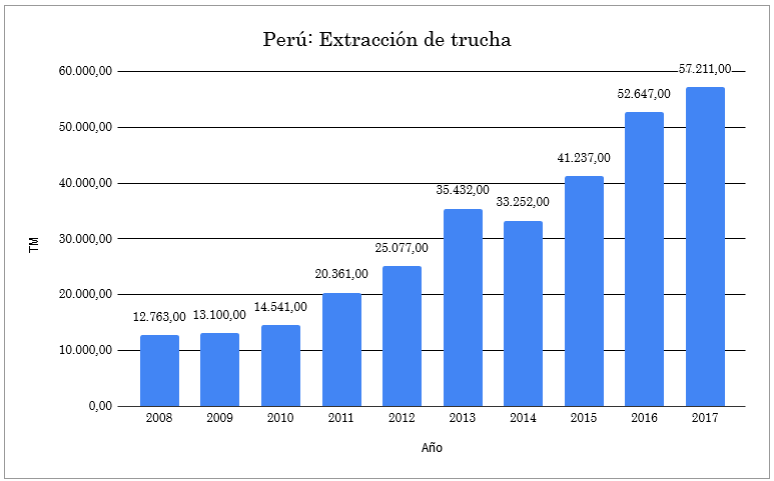
\includegraphics[width=1\textwidth]{chapter1/extraccion trucha toneladas anuales.png}
	\caption{Título de la figura que sale en el index y aquí.}
	 Datos: \citep{MinisteriodelaProducciondelPeru2018} 	 \\ 
	 Gráfico: Elaboración propia.
	\label{fig:nombre llave para referenciar la imagen en el texto}
\end{figure}

Así puedes citar la imagen: Figura \ref{fig:nombre llave para referenciar la imagen en el texto}.

Se puede citar a autores con tipografía asiática : \citep{2010}

Una tabla puedes presentarla como imagen de forma sencilla o realizarla en lenguaje LaTeX. Cómo incluir imagenes ya lo explicamos. 

En LaTeX existen dos tipos de tablas: las tablas normales representadas por la palabra clave "table" y las tablas que pueden separarse si abarcan más de una página conservando su cabecera (Se especifica la cabecera de la tabla).

Todas estas tablas no tienen que ser llenadas a mano, pueden generarse con la ayuda de páginas webs.

%% NUEVA SUB-SUB-SECCION X.X.X.X
\subsubsection{Tabla simple}

- Sirve para mostrar tablas de forma sencilla
- No se separa manteniendo encabezado.
- No se puede poner dentro de la tabla referencias a pie de página
- 



% Please add the following required packages to your document preamble:
% \usepackage[table,xcdraw]{xcolor}
% If you use beamer only pass "xcolor=table" option, i.e. \documentclass[xcolor=table]{beamer}
\begin{table}[H]
	\centering
	\caption{Comparación entre los métodos de clasificación.}
	\label{tbl:comparacion entre metodos de clasificacion}
	\begin{tabular}{|l|c|c|c|c|}
		\hline
		\rowcolor[HTML]{A6A6A6} 
		\multicolumn{1}{|c|}{\cellcolor[HTML]{A6A6A6}{\color[HTML]{000000} \textbf{Criterio\textbackslash{}Método}}} & {\color[HTML]{000000} \textbf{Manual}} & {\color[HTML]{000000} \textbf{Mecánico}} & {\color[HTML]{000000} \textbf{\begin{tabular}[c]{@{}c@{}}Visión por\\  computadora\end{tabular}}} & {\color[HTML]{000000} \textbf{\begin{tabular}[c]{@{}c@{}}Inteligencia \\ Artificial\end{tabular}}} \\ \hline
		{\color[HTML]{000000} \begin{tabular}[c]{@{}l@{}}Cantidad de peces \\ por hora\end{tabular}} & {\color[HTML]{000000} \begin{tabular}[c]{@{}c@{}}120\\ (por operario)\end{tabular}} & {\color[HTML]{000000} 18000} & {\color[HTML]{000000} \begin{tabular}[c]{@{}c@{}}Según capacidad \\ de cómputo\end{tabular}} & {\color[HTML]{000000} \begin{tabular}[c]{@{}c@{}}Según capacidad\\ de cómputo\end{tabular}} \\ \hline
		{\color[HTML]{000000} Mantenimiento} & {\color[HTML]{000000} -} & {\color[HTML]{000000} Semestral} & {\color[HTML]{000000} Anual} & {\color[HTML]{000000} Anual} \\ \hline
		{\color[HTML]{000000} \begin{tabular}[c]{@{}l@{}}Costo de \\ implementación\end{tabular}} & {\color[HTML]{000000} Bajo} & {\color[HTML]{000000} Medio} & {\color[HTML]{000000} Medio} & {\color[HTML]{000000} Medio} \\ \hline
		{\color[HTML]{000000} \begin{tabular}[c]{@{}l@{}}Costo de \\ funcionamiento\end{tabular}} & {\color[HTML]{000000} Bajo} & {\color[HTML]{000000} Bajo} & {\color[HTML]{000000} Medio} & {\color[HTML]{000000} Alto} \\ \hline
		{\color[HTML]{000000} Precisión} & {\color[HTML]{000000} Media} & {\color[HTML]{000000} Alta} & {\color[HTML]{000000} Alta} & {\color[HTML]{000000} Muy alta} \\ \hline
	\end{tabular}
	\\ Fuente: Elaboración Propia.
\end{table}

%% NUEVA SUB-SUB-SECCION X.X.X.X
\subsubsection{Tabla simple con 1 imagen dentro}

\begin{table}[H]
	\centering	
	\caption{Comercio internacional de productos pesqueros por principales importadores y exportadores en miles de dólares.}
	\label{tbl:comercio internacional de productos pesqueros por principales importadores y exportadores en dolares}
	\begin{tabular}{ l }
		\begin{minipage}{1\textwidth}
			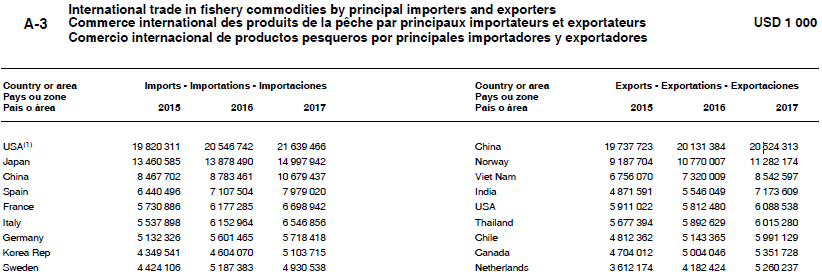
\includegraphics[width=1\textwidth]{chapter1/comercio internacional de productos pesqueros por principales importadores y exportadores en dolares.png}
		\end{minipage}	
	\end{tabular}
	\\	Fuente: FAO.
\end{table}


%% NUEVA SUB-SUB-SECCION X.X.X.X
\subsubsection{Tabla simple con algunos bordes en blanco y columnas combinadas}


% Please add the following required packages to your document preamble:
% \usepackage[table,xcdraw]{xcolor}
% If you use beamer only pass "xcolor=table" option, i.e. \documentclass[xcolor=table]{beamer}
\begin{table}[H]
	\centering	
	\caption{Clasificación de truchas por etapas de producción.}
	\label{tbl:clasificacion de truchas por etapas de produccion}
	\begin{tabular}{l|c|c|c|c|c|c|c|c|c|}
		\cline{2-10}
		& \cellcolor[HTML]{9B9B9B}{\color[HTML]{000000} \textbf{\rot{Siembra}}} & \cellcolor[HTML]{9B9B9B}{\color[HTML]{000000} \textbf{\rot{Alevinaje I}}} & \cellcolor[HTML]{9B9B9B}{\color[HTML]{000000} \textbf{\rot{Alevinaje II}}} & \cellcolor[HTML]{9B9B9B}{\color[HTML]{000000} \textbf{\rot{Alevinaje III}}} & \cellcolor[HTML]{9B9B9B}{\color[HTML]{000000} \textbf{\rot{Juvenil I}}} & \cellcolor[HTML]{9B9B9B}{\color[HTML]{000000} \textbf{\rot{Juvenil II}}} & \cellcolor[HTML]{9B9B9B}{\color[HTML]{000000} \textbf{\rot{Engorde I}}} & \cellcolor[HTML]{9B9B9B}{\color[HTML]{000000} \textbf{\rot{Engorde II}}} & \cellcolor[HTML]{9B9B9B}{\color[HTML]{000000} \textbf{\rot{Cosecha}}} \\ \hline
		\multicolumn{1}{|l|}{\cellcolor[HTML]{9B9B9B}\textbf{De \textit{(mm)}}} & - & 35 & 51 & 81 & 121 & 141 & 171 & 201 & 261 \\ \hline
		\multicolumn{1}{|l|}{\cellcolor[HTML]{9B9B9B}\textbf{Hasta \textit{(mm)}}} & 34 & 50 & 80 & 120 & 140 & 170 & 200 & 260 & - \\ \hline
		\multicolumn{1}{|l|}{\cellcolor[HTML]{9B9B9B}\textbf{De \textit{(g)}}} & - & 2.81 & 6.91 & 11 & 51 & 110 & 153 & 200 & 251 \\ \hline
		\multicolumn{1}{|l|}{\cellcolor[HTML]{9B9B9B}\textbf{Hasta \textit{(g)}}} & 2.80 & 6.90 & 10 & 50 & 109 & 152 & 199 & 250 & 290 \\ \hline
		\multicolumn{1}{|l|}{\cellcolor[HTML]{9B9B9B}\textbf{Este trabajo \textit{(mm)}}} & \multicolumn{3}{c|}{} & \multicolumn{4}{c|}{\cellcolor[HTML]{C0C0C0}100 a 200} & \multicolumn{2}{c|}{} \\ \hline
	\end{tabular}
	\\Fuente: FONDEPES.
\end{table}

%% NUEVA SUB-SUB-SECCION X.X.X.X
\subsubsection{Tabla simple con ajuste al texto y no al borde de la página}

% Please add the following required packages to your document preamble:
% \usepackage[table,xcdraw]{xcolor}
% If you use beamer only pass "xcolor=table" option, i.e. \documentclass[xcolor=table]{beamer}
\begin{table}[H]	
	\centering
	\caption{Comparación entre los métodos de traslado de peces.}
	\label{tbl:comparacion entre los metodos de traslado de peces}
	\begin{tabular}{|
			>{\columncolor[HTML]{D9D9D9}}l |c|c|}
		\hline
		\multicolumn{1}{|c|}{\cellcolor[HTML]{A6A6A6}{\color[HTML]{000000} \textbf{Criterio\textbackslash{}Método}}} &
		\cellcolor[HTML]{A6A6A6}{\color[HTML]{000000} \textbf{Manual}} &
		\cellcolor[HTML]{A6A6A6}{\color[HTML]{000000} \textbf{Automático}} \\ \hline
		{\color[HTML]{000000} Cantidad de peces por hora} &
		{\color[HTML]{000000} \begin{tabular}[c]{@{}c@{}}360 aproximadamente\\ (por operario)\end{tabular}} &
		{\color[HTML]{000000} 20000} \\ \hline
		{\color[HTML]{000000} Mantenimiento}           & {\color[HTML]{000000} -}    & {\color[HTML]{000000} Semestral} \\ \hline
		{\color[HTML]{000000} Costo de implementación} & {\color[HTML]{000000} Bajo} & {\color[HTML]{000000} Alto}      \\ \hline
		{\color[HTML]{000000} Costo de funcionamiento} & {\color[HTML]{000000} Bajo} & {\color[HTML]{000000} Alto}      \\ \hline
		{\color[HTML]{000000} Precisión}               & {\color[HTML]{000000} Bajo} & {\color[HTML]{000000} Medio}     \\ \hline
	\end{tabular}
	\\ Fuente: Elaboración propia.
\end{table}
 

%% NUEVA SUB-SUB-SECCION X.X.X.X
\subsubsection{Tabla simple que si acepta pie de página dentro}


% Please add the following required packages to your document preamble:
% \usepackage[table,xcdraw]{xcolor}
% If you use beamer only pass "xcolor=table" option, i.e. \documentclass[xcolor=table]{beamer}
\begin{savenotes}
	\begin{table}[H]
		\centering
		\caption{Comparación de clasificadores comerciales.}
		\label{tbl:comparacion de clasificadores comerciales}
		\begin{tabular}{|
			>{\columncolor[HTML]{D9D9D9}}l |c|c|c|c|}
			\hline
			\multicolumn{1}{|c|}{\cellcolor[HTML]{A6A6A6}{\color[HTML]{000000} \textbf{Criterio\textbackslash{}Método}}} &
			\cellcolor[HTML]{A6A6A6}{\color[HTML]{000000} \textbf{AGK}} &
			\cellcolor[HTML]{A6A6A6}{\color[HTML]{000000} \textbf{HELIOS 25\footnote{También existe Helios 10, 30, 40, 50, 60 y 100. En el Anexo A2 se muestra las características de cada una.}}} &
			\cellcolor[HTML]{A6A6A6}{\color[HTML]{000000} \textbf{APOLLO}} &
			\cellcolor[HTML]{A6A6A6}{\color[HTML]{000000} \textbf{\begin{tabular}[c]{@{}c@{}}PENTAIR\\ V-10000140\footnote{Cotización a empresa Pentair en el Anexo A3.}\end{tabular}}} \\ \hline
			{\color[HTML]{000000} Compra} &
			{\color[HTML]{000000} \begin{tabular}[c]{@{}c@{}}Depende\\ del stock\end{tabular}} &
			{\color[HTML]{000000} \begin{tabular}[c]{@{}c@{}}Depende\\ del stock\end{tabular}} &
			{\color[HTML]{000000} \begin{tabular}[c]{@{}c@{}}Depende\\ del stock\end{tabular}} &
			{\color[HTML]{000000} A pedido\footnote{Diseño y envío de 6 a 8 semanas luego de ordenar y realizar el pago. Las especificaciones se indican luego de diseñado el producto.}} \\ \hline
			{\color[HTML]{000000} Rango ($ g $)} &
			{\color[HTML]{000000} 10 a 200} &
			{\color[HTML]{000000} 5 a 400} &
			{\color[HTML]{000000} \begin{tabular}[c]{@{}c@{}}1 a 650\\ 5 a 750\end{tabular}} &
			{\color[HTML]{000000} 0.5 a 200} \\ \hline
			{\color[HTML]{000000} Entradas} &
			{\color[HTML]{000000} 1} &
			{\color[HTML]{000000} 1} &
			{\color[HTML]{000000} 1} &
			{\color[HTML]{000000} 1} \\ \hline
			{\color[HTML]{000000} Salidas} &
			{\color[HTML]{000000} 4} &
			{\color[HTML]{000000} 6} &
			{\color[HTML]{000000} 4} &
			{\color[HTML]{000000} -} \\ \hline
			{\color[HTML]{000000} Capacidad por hora} &
			{\color[HTML]{000000} 70 000} &
			{\color[HTML]{000000} 95 000} &
			{\color[HTML]{000000} 95 000} &
			{\color[HTML]{000000} -} \\ \hline
			{\color[HTML]{000000} Potencia} &
			{\color[HTML]{000000} 0.15 kW} &
			{\color[HTML]{000000} 0.37 kW} &
			{\color[HTML]{000000} 0.18 kW} &
			{\color[HTML]{000000} -} \\ \hline
			{\color[HTML]{000000} RPM} &
			{\color[HTML]{000000} -} &
			{\color[HTML]{000000} -} &
			{\color[HTML]{000000} 900} &
			{\color[HTML]{000000} -} \\ \hline
			{\color[HTML]{000000} \begin{tabular}[c]{@{}l@{}}Suministro eléctrico\\ ($ V-Hz. $)\end{tabular}} &
			{\color[HTML]{000000} \begin{tabular}[c]{@{}c@{}}220/380   VAC \\ 50/60   Hz.\end{tabular}} &
			{\color[HTML]{000000} \begin{tabular}[c]{@{}c@{}}230   VAC\\ 50/60   Hz.\end{tabular}} &
			{\color[HTML]{000000} \begin{tabular}[c]{@{}c@{}}230/400\\ VAC  50 Hz.\end{tabular}} &
			{\color[HTML]{000000} \begin{tabular}[c]{@{}c@{}}220/230\\ VAC 60 Hz.\end{tabular}} \\ \hline
			{\color[HTML]{000000} Recepción de peces} &
			{\color[HTML]{000000} \begin{tabular}[c]{@{}c@{}}Manual /\\ Bombeo\\de peces\end{tabular}} &
			{\color[HTML]{000000} \begin{tabular}[c]{@{}c@{}}Manual /\\  Bombeo\\de peces\end{tabular}} &
			{\color[HTML]{000000} \begin{tabular}[c]{@{}c@{}}Manual /\\ Bombeo\\de peces\end{tabular}} &
			{\color[HTML]{000000} \begin{tabular}[c]{@{}c@{}}Bombeo\\ de peces\end{tabular}} \\ \hline
			{\color[HTML]{000000} \begin{tabular}[c]{@{}l@{}}Mínima velocidad de \\ entrada de caudal ($ m^3/h $)\end{tabular}} &
			{\color[HTML]{000000} -} &
			{\color[HTML]{000000} 40} &
			{\color[HTML]{000000} \begin{tabular}[c]{@{}c@{}}Bombeo\\de peces\end{tabular}} &
			{\color[HTML]{000000} -} \\ \hline
			{\color[HTML]{000000} Dimensiones ($ cm $)\footnote{Las dimensiones de la máquina son de largo($ l $), ancho($ a $) y alto($ h $).}} &
			{\color[HTML]{000000} 350x100x118} &
			{\color[HTML]{000000} 200x100x110\footnote{Altura ajustable de 110 a 140 $ cm $.}} &
			{\color[HTML]{000000} 315x128x128\footnote{Altura ajustable de 128 a 145 $ cm $.}} &
			{\color[HTML]{000000} -} \\ \hline
			{\color[HTML]{000000} Peso ($ kg $)} &
			{\color[HTML]{000000} 150} &
			{\color[HTML]{000000} 210} &
			{\color[HTML]{000000} 375} &
			{\color[HTML]{000000} -} \\ \hline
			{\color[HTML]{000000} Precisión ($ \% $)} &
			{\color[HTML]{000000} -} &
			{\color[HTML]{000000} 97} &
			{\color[HTML]{000000} -} &
			{\color[HTML]{000000} 97} \\ \hline
			{\color[HTML]{000000} Precio ($ \$ $)} &
			{\color[HTML]{000000} -} &
			{\color[HTML]{000000} -} &
			{\color[HTML]{000000} 15 730} &
			{\color[HTML]{000000} 53 567} \\ \hline
		\end{tabular}
	\\Fuente: AGK, Helios 25, Apollo, Pentair y Elaboración propia.
	\end{table}
\end{savenotes}
